

In this class, we relax the assumption that
the data points are independently and identically distributed (i.i.d.) 
by moving to a scenario of \emph{structured prediction}, where the inputs are assumed to have
temporal or spacial dependencies. We start by 
considering sequential models, which correspond to a \emph{chain structure}: for instance,
the words in a sentence. In this lecture, we will use part-of-speech
tagging as our example task.  

We focus on the well known Hidden Markov Model (HMM) on section
\ref{hmm}, where we describe how to estimate its parameters from labeled data
\ref{ml}. We will then move to how to find the most likely hidden sequence
(decoding) given an observation sequence and a parameter set
\ref{decoding}. This section will explain the required inference
algorithms (Viterbi and Forward-Backward) for sequence models. These
inference algorithms will be fundamental for the rest of this lecture,
as well as for the next lecture on \emph{discriminative} training of sequence
models. Section \ref{pos-tagging} will describe the task of 
part-of-speech tagging, and how HMM are suitable for this task. 
Finally, Section \ref{sec:em} will 
address unsupervised learning of HMMs through the EM
algorithm.


\section{Notation}

The problem setting is the following. 
We assume a finite set of \emph{observation labels}, 
$\vocab := \{w_1,\ldots,w_J\}$,
and a finite set of \emph{state labels}, 
$\statevocab := \{c_1,\ldots, c_K\}$.
In part-of-speech tagging, $\vocab$ is a 
vocabulary of word types, and 
$\statevocab$ is the set of part-of-speech tags 
(noun, verb, adjective, \emph{etc.})
Let $\varepsilon$ denote the empty string. 
We denote by 
$\vocab^* := \{\varepsilon\} \cup \vocab \cup \vocab^2 \cup \ldots$ and 
$\statevocab^* := \{\varepsilon\} \cup \statevocab \cup \statevocab^2  \cup \ldots$ the Kleene closure 
of each of the two sets above. 
Elements of $\vocab^*$ and $\statevocab^*$ 
are \emph{strings of observations} and \emph{strings of states}, 
respectively. 
Throughout this class, we 
assume our input set is $\X = \vocab^*$, 
and our output set is $\Y = \statevocab^*$. 
In other words, 
our inputs are observation sequences, 
$x = x_1 x_2 \ldots x_N$, 
for some $N \in \mathbb{N}$, where each $x_i \in \vocab$;
given such a $x$, we seek 
the corresponding state sequence, 
$y = y_1 y_2 \ldots y_N$, 
where each $y_i \in \statevocab$.
We will assume two scenarios in this lab:
\begin{enumerate}
\item \emph{Supervised learning.} We will 
train models from a sample set of paired observation and state sequences, $\mathcal{D}_L := \{(x^1,y^1), \ldots, (x^M,y^M)\} \subseteq \X \times \Y$.
\item \emph{Unsupervised learning.} We will also
train models from the set of observations only, $\mathcal{D}_U := \{x^1, \ldots, x^M\} \subseteq \X$.
\end{enumerate}
Our notation is summarized in Table~\ref{tab:hmm_notation}.

%Let $\X = \{\sent^1, \ldots, \sent^D\}$ be a training set of independent
%and identically-distributed random variables. In this work $\sent^d$
%(for notation simplicity we will drop the superscript $d$ when
%considering an isolated example) corresponds to a sentence in natural
%language and decomposes as a sequence of observations of length $N$: $\sent = \obs_1 \ldots
%\obs_N$. Each $\obs_n$ is a discrete
%random variable (a \emph{word}),  taking a value $\vv$ from a
%finite vocabulary $\vocab$. Each $\sent$ has an unknown hidden
%structure $\hseq$  that we want to predict. The
%structures are sequences $\hseq = \hs_1 \ldots \hs_N$ of the same
%length $N$ as the observations. Each hidden state $\hs_n$ is a discrete
%random variable and can take a value $\hv$ from a discrete vocabulary $\hvocab$. 
%
%\afm{need to improve notation}

\begin{table}[h]
\begin{center}
\begin{tabular}{|l|l|}
\hline
\multicolumn{2}{|c|}{Notation}\\
\hline
\hline
$\mathcal{D}_L$ & training set (including labeled data)\\
\hline
$\mathcal{D}_U$ & training set (unlabeled data only)\\
\hline
$M$  & number of training examples \\
\hline
$x = x_1 \ldots x_N$  & observation sequence \\
\hline
$y = y_1 \ldots y_N$  & state sequence \\
\hline
$N$  & length of the sequence \\
\hline
$x_i$ &  observation at position $i$ in the sequence\\
\hline
$y_i$ &  state at position $i$ in the sequence\\
\hline
${\tt start}, {\tt stop}$ & start and stop symbols\\
\hline
$\vocab$ & observation set\\
\hline 
$J$ & number of distinct observation types\\
\hline 
$w_j$ & particular observation, $j \in \{1,\ldots,J\}$\\
\hline 
$\statevocab$ & state set\\
\hline 
$K$ & number of distinct states\\
\hline 
$c_k$ & particular state, $k \in \{1,\ldots,K\}$\\
\hline  
\end{tabular}
\end{center}
\label{tab:hmm_notation}
\caption{General notation used in this class}
\end{table}








\section{\label{hmm} Hidden Markov Models}

The Hidden Markov Model (HMM) is one of the most common sequence
probabilistic models, and has been applied to a wide variety of
tasks. More generally, an HMM is a particular instance of  a chain
directed probabilistic graphical model, or a Bayesian network.  In a
Bayesian network, every random variable is represented as a node in a
graph, and the edges in the graph are directed and represent
probabilistic dependencies between the random variables. For an HMM, the random variables are divided into two sets, the 
\emph{observed} variables, in our case 
$\obs$, and the \emph{hidden} variables, in our case $\hs$. In the HMM
terminology, the observed variables are called \emph{observations}, and the
hidden variables are called \emph{states}. 

As you may find out in today's lab session, 
implementing the inference routines of the HMM can be challenging, 
and debugging can become hard in large
datasets. We thus start with a small and very
simple (very unrealistic!) example. The idea is that you may compute the desired
quantities by hand and check if your implementation yields the correct result. 

\begin{example}

Consider a person, which is only interested in four activities: 
\begin{itemize}
\item walking in
the park (w);
\item shopping (s);
\item cleaning his apartment (c);
\item playing tennis (t).
\end{itemize}
The choice of what to do on a given day is determined exclusively by the weather at that day. The
weather can be either \emph{rainy} (r) or \emph{sunny} (s). 
Now, suppose that we observe what the person did on a sequence of days; 
can we use that information to predict the weather each of those days? 
To tackle this problem, we assume 
that the weather behaves as a discrete Markov Chain: the weather on a
given day is independent of everything else \emph{given 
the weather on the previous day}. The entire system is that of a hidden Markov model (HMM).

Assume we are asked to predict what was the weather on two different
sequences of days given the following observations: ``walk walk shop
clean''  and ``clean walk tennis walk''. This will be our test set. 


To train our model, we will be given access to three different sequences of
days, containing both the activities and the weather on those days, namely: 
``walk/rainy walk/sunny shop/sunny
clean/sunny'', ``walk/rainy walk/rainy shop/rainy clean/rainy '' and ``shop/rainy walk/rainy shop/rainy clean/rainy''. This
will be our training set.
 \end{example}

Figure \ref{hmm} show the HMM model the first sequence of our simple
example (the notation is summarized in Table \ref{tab:hmm-simple-notation}).


\begin{table}[h]
\begin{center}
\begin{tabular}{|l|l|}
\hline
\multicolumn{2}{|c|}{HMM Example}\\
\hline
\hline
$\sent$ & observed sentence ``w w s c'' \\
\hline
$N = 4$ & observation length \\
\hline
$i,j$ & positions in the sentence: $i,j \in \{1 \ldots N\} $\\
\hline
$\vocab = \{w,s,c,t\}$ & observation vocabulary \\
\hline 
$p,q$ & indexes into the vocabulary $p,q \in |\vocab|$\\
\hline
$\obs_i = \vv_q,\obs_j = \vv_p$ & observation at position $\obs_i$ ($\obs_j$) has value $\vv_q$ ($\vv_p$)\\
\hline 
$\hvocab = \{r,s\}$ & hidden values vocabulary\\
\hline 
$l,m$ & indexes into the hidden values vocabulary\\
\hline
$\hs_i = \hv_l,\hs_j = \hv_m$ & state at position $\hs_i$ ($\hs_j$) has hidden value $\hv_l$ ($\hv_m$)\\
\hline
\end{tabular}
\end{center}
\caption[HMM notation]{\label{tab:hmm-simple-notation} HMM notation for the running example.}
\end{table}

\begin{figure}[ht]
\centering
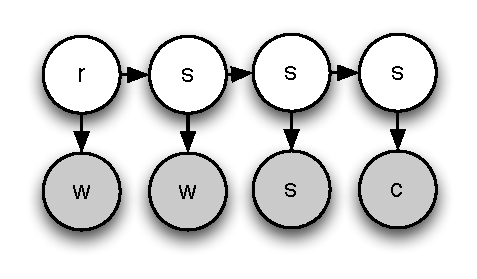
\includegraphics[scale=1]{figs/sequences/hmm}
\caption[HMM running example]{\label{fig:hmm} HMM structure, for the simple
running example.}
\end{figure}


A first order HMM model has the following independence assumptions over the joint distribution $\joint$:
\begin{itemize}
  \item \textbf{Independence of previous states.} The probability of
    being in a given state $\hv_l$ at position $\hs_i$ only depends on
    the state $\hv_m$ of the previous position $\hs_{i-1}$, that is 
    $p_{\theta} (\hs_i = \hv_l \mid \hs_{i-1} = \hv_m, \hs_{i-2} \ldots \hs_{1}) = p_{\theta} (\hs_i = \hv_l \mid \hs_{i-1} = \hv_m)$, 
    defining a first order Markov chain.%
    \footnote{The order of the Markov chain depends on the number of previous positions taken into account. 
    The remainder of the exposition can be easily extend to higher order HMM, giving the model more expressiveness, 
    but making inference harder.}
  \item \textbf{Homogeneous transition.} The probability of
    making a transition from state $\hv_l$ to state $\hv_m$ is independent of
    the particular position in the sentence, for all $i,j \in \{1,\ldots,N\}$:
    $p_{\theta} (\hs_i = \hv_l \mid \hs_{i-1} = \hv_m) =  p_{\theta}
    (\hs_j = \hv_l \mid \hs_{j-1} = \hv_m)$, so
    $p_{\theta} (\hs_i = \hv_l \mid \hs_{i-1} = \hv_m) = p_{\theta} (\hv_l \mid \hv_m)$.
  \item \textbf{Observation independence.}  The probability of
    observing $\vv_q$ at position $i$ is fully determined by the state
    at that position, that is  $p_{\theta}(\obs_i = \vv_q\mid
    \hs_i=\hv_l)$, and this probability is independent of the
    particular position, that is  $p_{\theta}(\obs_i = \vv_q\mid
    \hs_i=\hv_l)  = p_{\theta}(\vv_q\mid \hv_l)$.
\end{itemize}
These conditional independence assumptions are crucial to allow
efficient inference, as will be described. We also need to define a \emph{start probability}, the probability of starting 
at state $\hv_l$. Furthermore, when
dealing with text, it is usual to break the homogeneous transition
for the last position, and model the final transitions as 
independent parameters.
 The four probability
distributions that define the HMM model are summarized in Table
\ref{tab:hmm-dist}. 
For each one
of them we will use a short notation to simplify the exposition.
\begin{table}[h]
\begin{center}
\begin{tabular}{|l|l|l|}
\hline
\multicolumn{3}{|c|}{HMM distributions}\\
\hline
Name & probability distribution & short notation \\
\hline
\textbf{initial probability} & $p_{\theta} (\hs_1 = \hv_l)$ & $\pi_{l}$\\
\hline
\textbf{final probability} & $p_{\theta} (\hs_T = \hv_l \mid
\hs_{T-1} = \hv_m)$ & $f_{m,l}$\\
\hline
\textbf{transition probability} & $p_{\theta} (\hs_i = \hv_l \mid
\hs_{i-1} = \hv_m)$ & $a_{m,l}$\\
\hline
\textbf{observation probability} & $p_{\theta}(\obs_i = \vv_q\mid \hs_i = \hv_l)$ & $b_l(\obs_i) $ \\
\hline
\end{tabular}
\end{center}
\caption[HMM probability distributions]{\label{tab:hmm-dist} HMM probability distributions.}
\end{table}

The joint distribution can be expressed as:
\begin{equation}
  \joint =\pi_{\hs_1}b_{\hs_1}(\obs_1) [\prod_{i=2}^{N-1}
  a_{\hs_{i-1},\hs_{i}} b_{\hs_{i}}(\obs_i)] f_{\hs_{N-1},\hs_N}b_{\hs_{N}}(\obs_N),
  \label{eqn:hmm}
\end{equation}
which for the example from Figure \ref{fig:hmm} is:
\begin{equation}
  \joint =\pi_{r} b_r("w") a_{r,s}b_s("w") a_{s,s}b_s("s") f_{s,s}b_s("c").
  \label{eqn:hmm_ex}
\end{equation}

In the next section we turn our attention to estimating the different
probabilities distributions of the model  $\pi_l$, $a_{m,l}$,
$f_{m,l}$ and $b_l(\obs_i)$.

\begin{exercise}
Load the simple sequence dataset:
From the ipython command line (Note start ipython from the \emph{code}
directory), create a simple sequence object and look at the training
and test set.
\begin{python}
 In[]: run readers/simple_sequence.py
 In[]: simple = SimpleSequence()
 In[]: simple.train
Out[]: [w/r w/s s/s c/s , w/r w/r s/r c/s , w/s s/s s/s c/s ]
 In[]: simple.test
Out[]: [w/r w/s s/s c/s , c/s w/s t/s w/s ] 
\end{python}
\end{exercise}
%%% Local Variables: 
%%% mode: latex
%%% TeX-master: "../../guide"
%%% End: 






\section{\label{ml} Finding the Maximum Likelihood Parameters}
%So far we have not committed to any form for the probability
%distributions $\pi_l$, $a_{m,l}$ and $b_l(\obs_i)$. In both applications
%addressed in this class, both the observations and the hidden
%variables are discrete. The most common approach is to model each of
%these probability distributions as multinomial distributions,
%summarized in Table \ref{tt:mult-params}. Note that the number of parameters of $a_{l,m}$ is $|\hvocab|(|\hvocab|+1)$ because of the special ``STOP'' symbol.

%\begin{table}
%\begin{center}
%\begin{tabular}{|c|c|c|c|}
%\hline
%short notation & probability distribution  & |parameters|& constraint \\
%\hline
%$\pi_j$ & $p_{\theta} (\hs_1 = \hv_j)$ & $|\hvocab|$ & $\sum_{\hv \in \hvocab} \pi_j = 1$;\\
%\hline
%$a_{l,m}$ & $p_{\theta} (\hs_i = \hv_l \mid \hs_{i-1} = \hv_m)$ & $|\hvocab|(|\hvocab|+1)$ &$\sum_{\hv_l \in \hvocab} a_{m,l} = 1$;\\
%\hline
%%$f_{l,m}$ & $p_{\theta} (\hs_N = \hv_l \mid \hs_{N-1} = \hv_m)$ & $(|\hvocab|-1)^2$ &$\sum_{\hv_l \in \hvocab} t_{m,l} = 1$;\\
%%\hline
%$b_q(l) $& $p_{\theta}(\obs_i = \vv_q\mid \hs_i = \hv_l)$  & $|\hvocab||\vocab|$ &$\sum_{\vv_q \in \vocab} b_q(l)  = 1$.\\
%\hline
%\end{tabular}
%\end{center}
%\caption[HMM multinomial parametrization]{\label{tt:mult-params}Multinomial parametrization of the HMM distributions.}
%\end{table}

One important problem in HMMs is to estimate the 
model parameters, \emph{i.e.}, 
the distributions depicted in Table~\ref{tab:hmm-dist}. 
We will refer to the set of all these parameters 
as $\theta$. 
In a supervised setting, the HMM model
is trained to maximize the joint log-likelihood of the data. Given a
dataset $\mathcal{D}_L$, the objective being optimized is:
\begin{equation}
\argmax_{\theta} \sum_{m=1}^M \log P_{\theta}(X=x^m,Y=y^m),
\end{equation}
where $P_{\theta}(X=x^m,Y=y^m)$ is given by Eq.~\ref{eqn:hmm}.

In some applications (\emph{e.g.} speech recognition) 
the observation variables are continuous, hence the emission distributions are real-valued (\emph{e.g.} mixtures of Gaussians).
In our case, both the state set and the observation set are discrete (and finite), therefore we use
multinomial distributions for the emission and 
transition probabilities. 
Multinomial distributions are attractive for several reasons: first of
all, they are easy to implement; secondly, the maximum likelihood estimation of the parameters has a simple closed form. The parameters are just
normalized counts of events that occur in the corpus (the same as the
Na\"{i}ve Bayes from previous class).

Given our labeled corpus $\mathcal{D}_L$, the estimation process consists of counting how
many times each event occurs in the corpus and normalize the counts to
form proper probability distributions. Let us define the following
quantities, called sufficient statistics, that represent the counts of
each event in the corpus:

\begin{align}
\mathbf{Initial \ Counts\!:}\;\;\;\;  &  C_{\mathrm{init}}(c_k) = \sum_{m=1}^M
\Ind (y^m_1 = c_k); \label{eq::initialCounts}\\
%
%\mathbf{Final \ Counts\!:}\;\;\;\;  &  fc(\hv_l,\hv _m) = \sum_{\trex} 
%\Ind (\hs_N = \hv_l \mid \hs_{N-1} = \hv_m); \label{eq::finalCounts}\\
%
\mathbf{Transition \ Counts\!:}\;\;\;\;  &  C_{\mathrm{trans}}(c_k,c_l) =
\sum_{m=1}^M  \sum_{i = 2}^{N}
\Ind (y^m_i = c_k \wedge y^m_{i-1} = c_l); \label{eq::transitionCounts}\\
%
\mathbf{Final \ Counts\!:}\;\;\;\;  &  C_{\mathrm{final}}(c_k) = \sum_{m=1}^M
\Ind (y^m_N = c_k); \label{eq::finalCounts}\\
%
\mathbf{Emission \ Counts\!:}\;\;\;\;  &  
C_{\mathrm{emiss}}(w_j,c_k) = \sum_{m=1}^M
\sum_{i = 1}^{N}
\Ind (x^m_i = w_j \wedge y^m_i = c_k); \label{eq::emissionCounts}
\end{align}
Here $y^m_i$,  the underscript denotes the state index position for a given sequence, and the superscript denotes the sequence index in the dataset, and the same applies for the observations.
Note that $\Ind$ is an indicator function that has the value 1 when the
particular event happens, and zero otherwise. In other words, the previous
equations go through the training corpus and count how
often each event occurs. For example, Eq.~\ref{eq::transitionCounts} counts how many times $c_k$ follows state $c_l$. Therefore, $C_{\mathrm{trans}}(\text{\tt sunny},\text{\tt rainy})$ contains the number of times that a sunny day followed a rainy day.

%
%: e.g. the word ``w'' appears with state
%``s'', or state ``s'' follows another state ``s'', or state ``s''
%begins the sentence.


After computing the counts, one can perform some sanity checks
to make sure the implementation is correct. Summing over all entries
of each count table we should observe the following:

\begin{itemize}
\item \textbf{Initial \ Counts\!:} -- Should sum to the number of
  sentences: $\sum_{k=1}^K C_{\mathrm{init}}(c_k) = M$
%\item \textbf{Final \ Counts\!:} - Should sum to the number of sentences.
\item \textbf{Transition/Final \ Counts\!:} -- Should sum to the number of
  tokens: 
  $\sum_{k,l=1}^K C_{\mathrm{trans}}(c_k,c_l) + \sum_{k=1}^K C_{\mathrm{final}}(c_k) = MN$
%   minus 2 times the number of sentences. Note that there are
%  N-1 edges for each sentence, and the last edge is being accounted by
%  the final transitions. So this leaves us with N-2 edges per sentence,
%  where N is the number of tokens in that sentence.
\item \textbf{Observation \ Counts\!:} -- Should sum to the number of tokens: $\sum_{j=1}^J\sum_{k=1}^K C_{\mathrm{emiss}}(w_j,c_k) = MN$.
\end{itemize}

Using the sufficient statistics (counts) the parameter estimates are: 
\begin{align}
  P_{\mathrm{init}}(c_k | \text{\tt start}) &=  \frac{C_{\mathrm{init}}(c_k)}{\sum_{l=1}^K
    C_{\mathrm{init}}(c_l)}\\
  P_{\mathrm{final}}(\text{\tt stop} | c_l) &=  \frac{C_{\mathrm{final}}(c_l)}{\sum_{k=1}^K
    C_{\mathrm{trans}}(c_k,c_l) + C_{\mathrm{final}}(c_l)}\\
  P_{\mathrm{trans}}(c_k | c_l) &=  \frac{C_{\mathrm{trans}}(c_k,c_l)}{\sum_{p=1}^K
    C_{\mathrm{trans}}(c_p,c_l) + C_{\mathrm{final}}(c_l)}\\
  P_{\mathrm{emiss}}(w_j | c_k) &=  \frac{C_{\mathrm{emiss}}(w_j,c_k)}{\sum_{q=1}^J
    C_{\mathrm{emiss}}(w_q,c_k)}
\end{align}


%\begin{exercise}
%Convince yourself that the sanity checks described above are true.
%Collect the counts from a supervised corpus using method
%\emph{collect\_counts\_from\_corpus} and use the provided function \emph{sanity\_check\_counts} to perform these checks on the counts table. 
%%\begin{python}
%% def sanity_check_counts(self,seq_list):
%%\end{python}
%
%\begin{python}
%>>> import sequences.hmm as hmmc
%>>> hmm = hmmc.HMM(simple.x_dict, simple.y_dict)
%>>> hmm.train_supervised(simple.train)
%>>> hmm.sanity_check_counts(simple.train)
%>>> print "Initial Probabilities:", hmm.initial_probs
%
%>>> print "Transition Probabilities:", hmm.transition_probs
%
%>>> print "Final Probabilities:", print 
%hmm.final_probs
%
%>>> print "Emission Probabilities", print hmm.emission_probs
%
%Initial counts match
%Final counts match
%Transition counts match
%Observations counts match
%\end{python}
%\end{exercise}



\begin{exercise}
The provided function \emph{train\_supervised} from the \emph{hmm.py} file implements the above parameter estimates.
%Implement a function that estimates the maximum likelihood
%estimates for the parameters given the corpus in the class HMM.
%The function header is in the hmm.py file. 
%\begin{python}
%def train_supervised(self,sequence_list):
%\end{python}
Run this function given the simple dataset above and look at the estimated probabilities. Are they correct? You can also check the variables ending in \emph{\_counts} instead of \emph{\_probs} to see the raw counts (for example, typing \emph{hmm.initial\_counts} will show you the raw counts of initial states). How are the counts related to the probabilities?

\begin{python}
>>> import lxmls.sequences.hmm as hmmc
>>> hmm = hmmc.HMM(simple.x_dict, simple.y_dict)
>>> hmm.train_supervised(simple.train)
>>> print "Initial Probabilities:", hmm.initial_probs
[ 0.66666667  0.33333333]
>>> print "Transition Probabilities:", hmm.transition_probs
[[ 0.5    0.   ]
 [ 0.5    0.625]]
>>> print "Final Probabilities:", hmm.final_probs
[ 0.     0.375]
>>> print "Emission Probabilities", hmm.emission_probs
[[ 0.75   0.25 ]
 [ 0.25   0.375]
 [ 0.     0.375]
 [ 0.     0.   ]]
\end{python}
\end{exercise}


%%% Local Variables: 
%%% mode: latex
%%% TeX-master: "../../guide"
%%% End: 




\section{\label{decoding} Finding the most likely sequence - Decoding}
Given the learned parameters and a new
observation sequence $x = x_1\ldots x_N$, we want to find the sequence of hidden states $y^* = y_1^* \ldots y_N^*$ that ``best'' explains it.
 This is called the \emph{decoding} problem. There are several ways to define what we mean by the ``best''
$y^*$, depending on our goal: for instance, we may want to minimize the probability of error
on each hidden
variable $Y_i$, or we may want to find the best assignment
to the sequence $Y_1\ldots Y_N$ as a whole. 
Therefore, finding the best sequence
can be accomplished through different approaches:

\begin{itemize}
\item A first approach, normally called \textbf{posterior decoding} or \textbf{minimum risk decoding}, consists
in picking the highest state posterior for each position $i$ in the sequence:
\begin{equation}
y_i^* = \argmax_{y_i \in \Lambda} P(Y_i=y_i | X_1=x_1,\ldots,X_N =x_N).
\end{equation}
%where $\gamma_i(\hs_i)$ is the posterior probability $P(\hs_i|\sent)$. 
Note, however, that this approach does not guarantee that the sequence $y^*=y_1^* \ldots y_N^*$ will be a
valid sequence of the model. For instance, there might be a transition
between two of the best state posteriors with probability zero. 

\item A second approach, called \textbf{Viterbi decoding}, consists in
picking the best global hidden state sequence: 
\begin{eqnarray}
y^* &=& \argmax_{y = y_1\ldots y_N} P(Y_1=y_1,\ldots, Y_N=y_N | X_1=x_1,\ldots,X_N =x_N)\nonumber\\
&=& \argmax_{y = y_1\ldots y_N} P(Y_1=y_1,\ldots, Y_N=y_N, X_1=x_1,\ldots,X_N =x_N).
\end{eqnarray}
\end{itemize}

Both approaches (which will be explained in Sections~\ref{posterior} and~\ref{viterbi}, respectively) rely on dynamic programming and make use of the
independence assumptions of the HMM model. Moreover, they use an alternative
representation of the HMM called a \emph{trellis}. 

A trellis unfolds all possible states for each position and it makes explicit the independence assumption: each position only
depends on the previous position. Here, each column represents a position in the sequence and each row represents a possible state. Figure \ref{fig:trellis} shows the
trellis for the particular example in Figure \ref{fig:hmm}. 

\begin{figure}[ht]
\centering
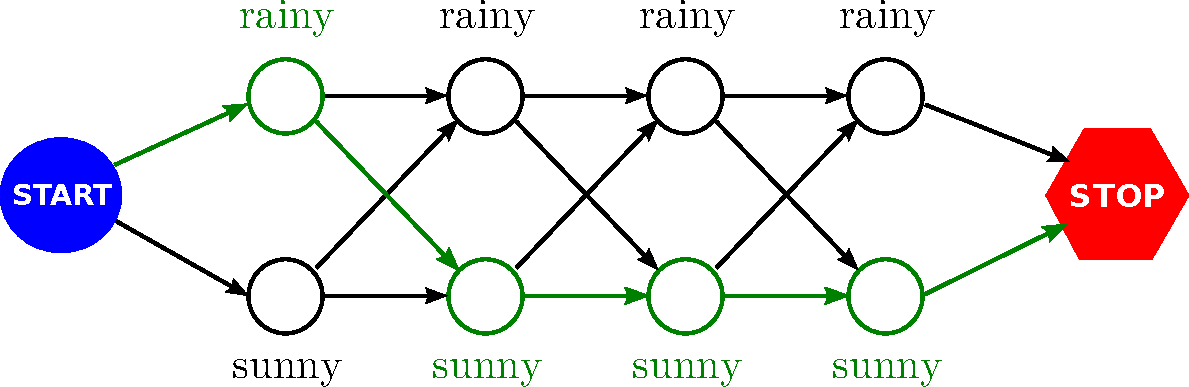
\includegraphics[width=0.7\textwidth]{figs/sequences/trellis_new}
\caption[HMM Trellis representation.]{\label{fig:trellis} Trellis
  representation of the HMM in Figure ~\ref{fig:hmm}, for the observation
  sequence ``{\tt walk} {\tt walk} {\tt shop} {\tt clean}'', where each hidden variable can take the values {\tt rainy} or {\tt sunny}.}
\end{figure}




Considering the trellis representation, note that we can include the following information:
\begin{itemize}
\item an \emph{initial probability} to the arrows that depart from the start symbol;
\item a \emph{final probability} to the arrows that reach the stop symbol;
\item a \emph{transition probability} to the remaining arrows; and,
\item an \emph{emission probability} to each circle, which is the probability that the observed symbol is emitted by that particular state.
\end{itemize}

For convenience, we will be working with 
log-probabilities, rather than probabilities.\footnote{This will be motivated further in Section~\ref{sec:logdomain}, where we describe 
how operations can be performed efficiently
in the log-domain.} Therefore, if we associate to each circle and arrow in
the trellis a score that corresponds
to the log-probabilities above, 
and if we define the score of a path
connecting the {\tt start} and  {\tt stop} symbols as
the sum of the scores of the circles and arrows
it traverses, 
then 
the goal of finding the most likely sequence of states (Viterbi decoding) corresponds to 
finding the path with the highest score.




%---since 
%we'll be multiplying a lot of probabilities, 
%we prevent underflowing by working in the log-domain. 

%For the decoding algorithms described in the following sections, 
%it is
%useful to define a re-parametrization of the model in equation \eqref{eqn:hmm}, in terms of
%node potentials $\phi_n(l)$ (associating a number to each box in Figure \ref{fig:trellis})
%and edge potentials $\phi_{n-1,n}(l,m)$ (associating a number to each edge in  Figure
%\ref{fig:trellis}). For our example, this re-parametrization is given by
%%
%\begin{equation}
%  \joint =\phi_1(r)\phi_1(r,s)\phi_2(s)\phi_2(s,s)\phi_3(s)\phi_3(s,s)\phi_4(s).
%  \label{eqn:hmm_ex_treelis}
%\end{equation}
%
%%\begin{equation}
%%  \joint =\phi_1(``w'',r)\phi_1(r,s)\phi_2(``w'',s)\phi_2(s,s)\phi_3(``s'',s)\phi_3(s,s)\phi_4(``c'',s).
%%  \label{eqn:hmm_ex_treelis}
%%\end{equation}
%
%In other words, to do this re-parameterization we need to find expressions for the potential variables, (the $\phi$'s) such that \eqref{eqn:hmm} and \eqref{eqn:hmm_ex_treelis} are equal. The solution is given by
%\begin{equation}
%\phi_{i-1,i}(l,m) = a_{l,m}
%\label{eq:nodes1}
%\end{equation}
%and
%\begin{equation}
%\phi_i(l) = 
%\begin{cases}
% b_{\obs_i}(l)\pi_l \quad\text{i = 1}\\
% b_{\obs_i}(l) \quad\text{i = 2,\ldots,N-1}\\
% b_{\obs_i}(l)a_{l,STOP} \quad\text{i = N}
% \label{eq:nodes2}
%\end{cases}
%\end{equation}


%\begin{itemize}
%\item\emph{Edge Potentials} - correspond to the transition parameters, with the exception of the
%edges into the last position that correspond to the final transition parameters.
%\item\emph{Node Potentials} - correspond to the observation
%parameters for a given state and the observation at that position.  The
%first position is the exception and corresponds to the
%product between the observation parameters for that state and
%the observation in that position with the initial parameters for that state. 
%\end{itemize}

%Although this re-parametrization simplifies the exposition, and will be
%used in these lectures, it is not necessarily very practical since we
%will be reproducing several values (for instance the transition
%parameters for each position).


The trellis scores are given by the following expressions:
\begin{itemize}
\item For each state $c_k$:
\begin{eqnarray}
\mathrm{score}_{\mathrm{init}}(c_k) &=&
\log P_{\mathrm{init}}(Y_{1} = c_k | \text{\tt start}).
\end{eqnarray}
\item For each position $i \in {1,\ldots,N-1}$ and each pair of states $c_k$ and $c_l$:
\begin{eqnarray}
\mathrm{score}_{\mathrm{trans}}(i, c_k, c_l) &=&
\log P_{\mathrm{trans}}(Y_{i+1} = c_k | Y_i = c_l).
\end{eqnarray}
\item For each state $c_l$:
\begin{eqnarray}
\mathrm{score}_{\mathrm{final}}(c_l) &=&
\log P_{\mathrm{final}}(\text{\tt stop} | Y_N = c_l).
\end{eqnarray}
\item For each position $i \in {1,\ldots,N}$ and state $c_k$:
\begin{eqnarray}
\mathrm{score}_{\mathrm{emiss}}(i, c_k) &=&
\log P_{\mathrm{emiss}}(X_i = x_i | Y_i = c_k).
\end{eqnarray}
\end{itemize}

In the next exercise, you will compute the trellis scores.

\begin{exercise}
Convince yourself that the score of a path in the trellis 
(summing over the scores above) is equivalent 
to the log-probability $\log P(X=x,Y=y)$, 
as defined in 
Eq.~\ref{eqn:hmm_ex}. 
Use the given function \emph{compute\_scores} on the first training sequence and confirm that the values are correct. You should get the same values as presented below.

%Implement a function that builds the node and edge potentials for a
%given sequence. The function head is in the \emph{hmm.py} file:

%\begin{python}
% def build_potentials(self,sequence):
%\end{python}
%
%Run this function for the first training sequence from the simple
%dataset and compare the results given (If the results are the same
%then you are ready to go).

\begin{python}
initial_scores, transition_scores, final_scores, emission_scores = hmm.compute_scores(simple.train.seq_list[0])
print initial_scores

[-0.40546511 -1.09861229]

print transition_scores

[[[-0.69314718        -inf]
  [-0.69314718 -0.47000363]]

 [[-0.69314718        -inf]
  [-0.69314718 -0.47000363]]

 [[-0.69314718        -inf]
  [-0.69314718 -0.47000363]]]

print final_scores

[       -inf -0.98082925]

print emission_scores

[[-0.28768207 -1.38629436]
 [-0.28768207 -1.38629436]
 [-1.38629436 -0.98082925]
 [       -inf -0.98082925]] 
\end{python}

Note that scores which are $-\infty$ (\texttt{-inf}) correspond
to zero-probability events. 
\end{exercise}

\subsection{Computing in log-domain}\label{sec:logdomain}

We will see that the decoding algorithms 
will need to multiply twice as many probability terms as 
the length $N$ of the sequence. 
This may cause underflowing problems 
when $N$ is large, since the nested multiplication of numbers smaller than 1
may easily become smaller than the machine precision. To avoid that
problem, \cite{rabiner} presents a scaled version of the decoding algorithms that avoids this problem.
An alternative, which is widely used, is computing
in the log-domain. That is, instead of 
manipulating probabilities, manipulate log-probabilities (the scores presented above). 
Every time we need to multiply probabilities, 
we can sum their log-representations, since:
\begin{equation}
\log(\exp(a) \times \exp(b)) = a+b.
\end{equation}
Sometimes, we need to \emph{add} probabilities. 
In the log domain, this requires us to compute 
\begin{equation}
\log(\exp(a) + \exp(b)) = a + \log(1 + \exp(b-a)),
\end{equation}
where we assume that $a$ is smaller than $b$.


\begin{exercise}
Look at the module {\tt sequences/log\_domain.py}. 
This module implements a function
{\tt logsum\_pair(logx, logy)} to 
add two numbers represented in the log-domain;
it returns their sum also represented in the log-domain. The function {\tt logsum(logv)} 
sums all components of an array 
represented in the log-domain. 
This will be used later in our decoding algorithms.
To observe why this is important, type the 
following:
\begin{python}
import numpy as np
a = np.random.rand(10)
np.log(sum(np.exp(a)))
2.8397172643228661

np.log(sum(np.exp(10*a)))
10.121099917705818

np.log(sum(np.exp(100*a)))
93.159220940569128

np.log(sum(np.exp(1000*a)))
inf

from lxmls.sequences.log_domain import *
logsum(a)
2.8397172643228665

logsum(10*a)
10.121099917705818

logsum(100*a)
93.159220940569114

logsum(1000*a)
925.88496219586864
\end{python}
\end{exercise}


\subsection{Posterior Decoding}\label{posterior}
Posterior decoding consists
in picking state with the highest posterior for each position in the sequence independently; for 
each $i = 1,\ldots,N$:
\begin{equation}
y_i^* = \argmax_{y_i \in \statevocab} P(Y_i=y_i | X = x).
\end{equation}
The \textbf{sequence posterior distribution} is the probability of a particular
hidden state sequence given that we have observed a particular
sequence. Moreover, we will be interested in two other posteriors distributions:
the \textbf{state posterior distribution}, corresponding to the
probability of being in a given state in a certain position given the
observed sequence; and the \textbf{transition posterior distribution},
which is the probability of making a particular transition, from position $i$ to
$i+1$, given the observed sequence. They are formally defined as follows:
\begin{align}
  \mathbf{Sequence \ Posterior\!:}\;\;\;\; &P(Y=y|X=x) = \frac{P(X=x,Y=y)}{P(X=x)}; \label{eq::posteriorDistribution} \\
 \mathbf{State \ Posterior\!:}\;\;\;\;  & P(Y_i=y_i | X=x); \label{eq::nodePosterior} \\
 \mathbf{Transition \ Posterior\!:}\;\;\;\;  &P(Y_{i+1}=y_{i+1},Y_i=y_i| X=x).\label{eq::edgePosterior}
\end{align}

To compute the posteriors, a first step is to be able to compute the 
likelihood of
the sequence $P(X=x)$, which corresponds to summing the probability of all
possible hidden state sequences.
\begin{equation}
\label{likelihoood}
\mathbf{Likelihood\!:}\;\;\;\; P(X=x) = \displaystyle \sum_{y \in \statevocab^N} P(X=x,Y=y).
\end{equation}
The number of possible hidden state sequences is exponential in the
length of the sequence ($|\statevocab|^N$),
 which makes the sum over all of them hard. 
 In our simple
 example, there are $2^4 = 16$ paths, which we can actually explicitly enumerate
 and calculate their probability using Equation \ref{eqn:hmm}. But this is as far as it goes: for example, for Part-of-Speech
 tagging with a small tagset of 12 tags and a medium size
 sentence of length 10, there are $12^{10} = 61 917 364 224$ such
 paths. 
Yet, we must be able to compute this sum (sum over $y \in \statevocab^N$) to compute the above likelihood
formula; this is called the inference problem. For sequence models, there is a well known dynamic programming algorithm,
the \textbf{Forward-Backward} (FB) algorithm, which allows the computation
to be performed in linear time,%
\footnote{The runtime is linear with respect
to the sequence length. More precisely, 
the runtime is $O(N|\statevocab|^2)$. 
A naive enumeration would cost $O(|\statevocab|^N)$.} %
by making use of the independence assumptions.

The FB algorithm relies on the independence of previous states
assumption, which  
is illustrated in the trellis view by having arrows only between consecutive states. 
The FB algorithm defines two auxiliary probabilities, the forward probability and the backward probability. 

\subsection*{Efficient forward probability computation}
The forward probability represents the probability that in position
$i$ we are in state $Y_i = c_k$ and that we have observed $x_1,\ldots,x_i$
up to that position. Therefore, its mathematical expression is:
\begin{equation}
\label{eq::forward}
\mathbf{Forward \ Probability\!:}\;\;\;\;  \mathrm{forward}(i, c_k) = P(Y_i = c_k, X_1=x_1,\ldots, X_i = x_i)
\end{equation}

Using the independence assumptions of the HMM we can compute $\mathrm{forward}(i, c_k)$ using all the forward computations \{$\mathrm{forward}(i -1, c)$ for $c \in \statevocab$\}. In order to facilitate the notation of the following argument we will denote by $x_{i:j}$  the assignemnt $X_i = x_i, \dots, X_j = x_j$. Therefore we can write   $\mathrm{forward}(i, y_i) $ as $P( y_i, x_{1:i } ) $ and rewrite the forward expression as follows:
\begin{equation}
\label{eq::forward2}
  P( y_i, x_{1:i } ) =  \sum_{y_{i-1} \in \statevocab} P( y_i ,y_{i-1}, x_{1:i } )  =  \sum_{y_{i-1} \in \statevocab} P( x_i  | y_i,  y_{i-1},  x_{1:i-1 } ) \cdot P(y_i  | y_{i-1},  x_{1:i-1 }) \cdot P(y_{i-1},  x_{1:i-1 })  
\end{equation}

Using the \textbf{Observation independence} and the \textbf{Independence of previous states} properties of the first order HMM we have $P( x_i  | y_i,  y_{i-1},  x_{1:i-1 } ) = P( x_i  | y_i) $ and $P(y_i  | y_{i-1},  x_{1:i-1 })  = P(y_i  | y_{i-1})  $. Therefore equation (\ref{eq::forward2}) can be written, 
for $i \in \{2,\dots,N\}$ (where $N$ is the length of the sequence), as 
\begin{equation}
\label{eq::forward3}
 \mathrm{forward}(i, y_i)  = \sum_{y_{i-1} \in \statevocab} P( x_i  | y_i, ) \cdot P(y_i  | y_{i-1}) \cdot \mathrm{forward}(i-1, y_{i-1})   
\end{equation}

 Using equation (\ref{eq::forward3}) we have proved that  the forward probability can be defined by the
following recurrence rule: 
\begin{eqnarray}
\mathrm{forward}(1, c_k)&=& P_{\mathrm{init}}(c_k|\text{\tt start}) \times 
P_{\mathrm{emiss}}(x_1 | c_k)
 \\
 \mathrm{forward}(i, c_k) &=& \left( \displaystyle \sum_{c_l \in \statevocab} P_{\mathrm{trans}}(c_k | c_l) \times \mathrm{forward}(i-1, c_l) \right) \times P_{\mathrm{emiss}}(x_i | c_k)  \label{forwardRecursion}
 \\
  \mathrm{forward}(N+1, \text{\tt stop}) &=& \sum_{c_l \in \statevocab} P_{\mathrm{final}}(\text{\tt stop} | c_l) \times \mathrm{forward}(N, c_l).
\end{eqnarray}

%\begin{figure}
%\begin{center}
%\begin{tabular}{cc}
%
%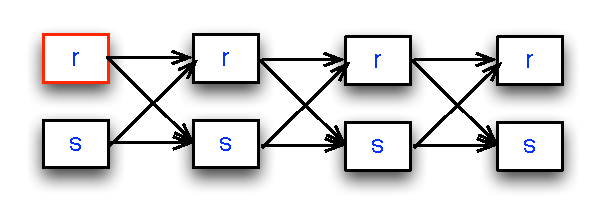
\includegraphics[scale=.5]{figs/sequences/forward1}
%& 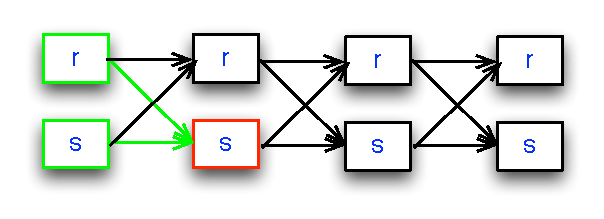
\includegraphics[scale=.5]{figs/sequences/forward2}\\
%\end{tabular}
%\caption[Forward-backward example.]{\label{fig:fb} Forward trellis for
%  the first sentence of the training data at position 1 (left) and at
%  position 2 (right)}
%
%\end{center}
%\end{figure}

%At position 1, the probability of being in state ``r'' and observing word ``w'' is just the node
%marginal for that position: $\alpha_1(r) = \phi_1(r)$ (see Figure
% \ref{fig:fb} left). At position 2 the probability
%of being in state ``s'' and observing the sequence of words ``w w''
%corresponds to the sum of all possible ways of reaching position 2 in
%state ``s'', namely, ``rs'' and ``ss'' (see Figure \ref{fig:fb} right). The probability of the former is
%$\phi_1(r)\phi_1(r,s)\phi_2(s)$
%and that of the latter is $\phi_1(s)\phi_1(s,s)\phi_2(s)$, so we get:
%\begin{eqnarray*}
%   \alpha_2(s) &=& \phi_1(r)\phi_1(r,s)\phi_2(s) +
%   \phi_1(s)\phi_1(s,s)\phi_2(s) \\
%   \alpha_2(s) &=& \left[\phi_1(r)\phi_1(r,s) +
%   \phi_1(s)\phi_1(s,s) \right]\phi_2(s) \\
% \alpha_2(s) &=& \displaystyle \sum_{\hs \in \hvocab}
% \left[\phi_1(\hs)\phi_1(\hs,s)\phi_2(s) \right] \\
%  \alpha_2(s) &=& \displaystyle \sum_{\hs \in \hvocab}
% \left[\alpha_1(\hs)\phi_1(\hs,s)\phi_2(s) \right]
%\end{eqnarray*}

Using the forward trellis one can compute the likelihood simply as:
\begin{equation}
\label{eq:forwardSum}
P(X=x) = \mathrm{forward}(N+1, \text{\tt stop}).
\end{equation}

Although the forward probability is enough to calculate the likelihood of a given sequence, we will also need the backward probability to calculate the state posteriors. 

% We could include a graph and comment the d-separation property which implies the conditional independence assumptions of the HMM graphically.
%\begin{figure}[ht]
%\centering
%\includegraphics[width=0.5\textwidth]{figs/sequences/hmm_diagram}
%\caption[HMM diagram]{\label{fig:hmm_diagram}Diagram showing the conditional independence relations of the HMM. If $Y_i$ is observed then...}
%\end{figure}

\subsection*{Efficient backward probability computation}

The backward probability is similar to the forward probability, but operates in the inverse direction.
It represents the probability of observing $x_{i+1},\ldots,x_N$ from position $i+1$ up to $N$, given that at position $i$ we are at state $Y_i = c_l$:
 \begin{equation}
\label{eq::backward}
\mathbf{Backward \ Probability\!:}\;\;\;\;  \mathrm{backward}(i, c_l) = P(X_{i+1}=x_{i+1},\ldots, X_N=x_N | Y_i = c_l).
\end{equation}

Using the independence assumptions of the HMM we can compute $\mathrm{backward}(i, c_k)$ using all the backward computations \{$\mathrm{backward}(i +1, c)$ for $c \in \statevocab$\}. Therefore we can write   $\mathrm{backward}(i, y_i) $ as $P( x_{i+1:N} | y_i ) $ and rewrite the forward expression as follows:
\begin{equation}
\label{eq::backward2}
  P( x_{i+1:N} | y_i ) =  \sum_{y_{i+1} \in \statevocab} P( x_{i+1:N}, y_{i+1} | y_i)  =  \sum_{y_{i+1} \in \statevocab} P( x_{i+2:N} | y_i, y_{i+1}, x_{i+1}) 
   P( x_{i+1}, |  y_{i+1},  y_{i}) P( y_{i+1} | y_i)
\end{equation}

Using the previous equation we have proved that the backward probability can be defined by the following recurrence rule:

\begin{eqnarray}
\mathrm{backward}(N, c_l) &=& P_{\mathrm{final}}(\text{\tt stop} | c_l) 
 \\
 \mathrm{backward}(i, c_l) &=&  \displaystyle \sum_{c_k \in \statevocab} P_{\mathrm{trans}}(c_k | c_l) \times \mathrm{backward}(i+1, c_k) \times P_{\mathrm{emiss}}(x_{i+1} | c_k)  \label{backwardRecursion}
 \\
  \mathrm{backward}(0, \text{\tt start}) &=& \sum_{c_k \in \statevocab} P_{\mathrm{init}}(c_k | \text{\tt start}) \times \mathrm{backward}(1, c_k) \times P_{\mathrm{emiss}}(x_{1} | c_k).
\end{eqnarray}
%At position $N$ there are no more observations, and the backward
%probability is set to 1. At position $i$, the probability 
%of having observed the future and being in state $\hv_l$, is given by the sum for all possible states of the probability of having transitioned 
%from position $i$ with state $\hv_l$ to position $i+1$ with state $\hv_m$, and observing $\obs_{i+1}$ at time $i+1$ and the future from there onward, which is $\beta_{i+1}(\hs_{i+1} = \hv_m)$. 
Using the backward trellis one can compute the likelihood simply as:.
\begin{equation}
\label{eq:backwardSum}
P(X=x) = \mathrm{backward}(0, \text{\tt start}).
\end{equation}

\subsection*{The forward backward algorithm}

We have seen how we can compute the probability of a sequence $x$ using the the forward and backward probabilities by computing  $\mathrm{forward}(N+1, \text{\tt stop})$ and $ \mathrm{backward}(0, \text{\tt start})$ respectively. Moreover,  the probability of a sequence $x$ can be computed with both forward and backward probabilities at a particular position $i$. The probability of a  given sequence $x$ at any position $i$ in the sequence can be computed
as follows \footnote{ The second equality in \ref{eq::fbsanity} can be justified as follows. Since $Y_i=y_i$ is observed then  $X_{i+1}, \dots, X_{N}$ is conditionally independent from any $X_k$ for $k \leq i$ . Therefore  $P(x_1,\dots, x_N, y_i) =  P( x_{i+1},\dots, x_N �| yi , x_1, \dots,x_i ) \cdot P( yi , x_1, \dots,x_i ) =  P( x_{i+1},\dots, x_N �| yi  ) \cdot P( yi , x_1, \dots,x_i ) = backward(i,y_i) \cdot forward(i,y_i)$.}:


\begin{eqnarray}
\label{eq::fbsanity}
  P(X=x) &=& 
  \sum_{c_k \in \statevocab} P(X_1=x_1,\ldots, X_N=x_N,Y_i=c_k)\nonumber\\
  & =&
  \sum_{c_k \in \statevocab} 
  \underbrace{P(X_1=x_1,\ldots, X_i=x_i, Y_i=c_k)}_{\mathrm{forward}(i,c_k)} \times 
  \underbrace{P(X_{i+1}=x_{i+1},\ldots, X_N=x_N| Y_i=c_k)}_{\mathrm{backward}(i,c_k)}\nonumber\\
  &=& \sum_{c_k \in \statevocab} \mathrm{forward}(i,c_k) \times \mathrm{backward}(i,c_k).
\end{eqnarray}


This equation will work for any choice of $i$. Although redundant, this fact is useful when implementing an
HMM as a sanity check that the computations are being performed
correctly, since one can compute this expression for several $i$; they should all yield the same value. 

Algorithm \ref{alg:fb} shows the pseudo code for the forward backward algorithm. The reader can notice that the $forward$ and $backward$ computations in the algorithm make use of $P_{emiss}$ and $P_{trans}$. There are a couple of details that should be taken into account if the reader wants to understand the algorithm using scores instead of probabilities.

% maybe more details on how to implement the algorithm using "scores" instead of probabilities should be given. 
\begin{itemize}
\item  $forward(i,\hat{c})$  is computed using $P_{emiss}(x_i | \hat{c})$ which does not depend on the sum over all possible states $c_k \in  \statevocab $. Therefore when taking the logarithm of the sum over all possible states the recurrence of the forward computations can be split as a sum of two logarithms.
\item $backward(i,\hat{c})$  is computed using $ P_{\mathrm{trans}}(c_k | \hat{c} )$ and $P_{\mathrm{emiss}}(x_{i+1} | c_k) $ both of  which  depend on $c_k$. Therefore when taking the logarithm of the sum the expression cannot be split as a sum of logarithms.
\end{itemize}


\begin{algorithm}[t]
   \caption{Forward-Backward algorithm \label{alg:fb}}
\begin{algorithmic}[1]
   \STATE {\bfseries input:} sequence $x_1,\ldots,x_N$, scores $P_{\mathrm{init}}, P_{\mathrm{trans}}, P_{\mathrm{final}}, P_{\mathrm{emiss}}$
        \item[]
        \STATE  \emph{Forward pass}: Compute the forward probabilities
        %\STATE \emph{Initialization}
        \FOR{$c_k \in \statevocab$ }
        \STATE $\mathrm{forward}(1,c_k) = P_{\mathrm{init}}(c_k|\text{\tt start}) \times 
P_{\mathrm{emiss}}(x_1 | c_k)$
        \ENDFOR 
        \FOR{$i=2$ {\bfseries to} $N$}
         \FOR{$\hat{c} \in \statevocab$ }
                 \STATE $\mathrm{forward}(i, \hat{c} ) = \left( \displaystyle \sum_{c_k \in \statevocab} P_{\mathrm{trans}}(\hat{c}| c_k) \times \mathrm{forward}(i-1, c_k) \right) \times P_{\mathrm{emiss}}(x_i | \hat{c})$
         \ENDFOR 
        \ENDFOR 
       \item[]
       \STATE \emph{Backward pass}: Compute the backward probabilities
      % \STATE \emph{Initialization}
        \FOR{$c_k \in \statevocab$ }
        \STATE $\mathrm{backward}(N, c_k) = P_{\mathrm{final}}(\text{\tt stop} | c_k)$
        \ENDFOR 
       \FOR{$i=N-1$ {\bfseries to} 1}
                 \FOR{$\hat{c} \in \statevocab$ }
       \STATE $\mathrm{backward}(i, \hat{c}) =  \displaystyle \sum_{c_k \in \statevocab} P_{\mathrm{trans}}(c_k | \hat{c} ) \times \mathrm{backward}(i+1, c_k) \times P_{\mathrm{emiss}}(x_{i+1} | c_k)$
       	 \ENDFOR 
        \ENDFOR 
        \item[]
       \STATE \textbf{output:} The forward and backward probabilities.
\end{algorithmic}
\end{algorithm}




\begin{exercise}
%Given the implementation of the forward pass of the forward backward
%algorithm in the file \emph{forward\_backward.py}, implement the backward pass.
%\begin{python}
%
%def forward_backward(node_potentials,edge_potentials):
%    H,N = node_potentials.shape
%    forward = np.zeros([H,N],dtype=float)
%    backward = np.zeros([H,N],dtype=float)
%    forward[:,0] = node_potentials[:,0]
%    ## Forward loop
%    for pos in xrange(1,N):
%        for current_state in xrange(H):
%            for prev_state in xrange(H):
%                forward_v = forward[prev_state,pos-1]
%                trans_v = edge_potentials[prev_state,current_state,pos-1]
%                prob = forward_v*trans_v
%                forward[current_state,pos] += prob
%            forward[current_state,pos] *= node_potentials[current_state,pos]
%    ## Backward loop
%          ## Your code
%   return forward,backward
%
%\end{python}

Run the provided forward-backward algorithm on the first train sequence. 
Observe that both the forward and the backward 
passes give the same log-likelihood.
%Use the provided function that makes use of Equation \ref{eq::fbsanity} to make
%sure your implementation is correct: 
\begin{python}
log_likelihood, forward = hmm.decoder.run_forward(initial_scores, transition_scores, final_scores, emission_scores)
print 'Log-Likelihood =', log_likelihood

Log-Likelihood = -5.06823232601

log_likelihood, backward = hmm.decoder.run_backward(initial_scores, transition_scores, final_scores, emission_scores)
print 'Log-Likelihood =', log_likelihood

Log-Likelihood = -5.06823232601
\end{python}
\end{exercise}


Given the forward and backward probabilities, one can compute both the state
and transition posteriors 
(you can hint why by looking at the term inside the sum in Eq.~\ref{eq::fbsanity}).


\begin{align}
 \mathbf{State \ Posterior\!:}\;\;\;\;  & P(Y_i = y_i| X=x) = \frac{\mathrm{forward}(i, y_i) \times 
 \mathrm{backward}(i, y_i)}{P(X=x)}; \label{eq::nodePosterior2} \\
 \mathbf{Transition \ Posterior\!:}\;\;\;\; &
 P(Y_i = y_i, Y_{i+1} = y_{i+1} | X=x)= \nonumber\\
 &
   \frac{\mathrm{forward}(i, y_i) \times 
   P_{\mathrm{trans}}(y_{i+1}|y_i) \times
   P_{\mathrm{emiss}}(x_{i+1}|y_{i+1}) \times
 \mathrm{backward}(i+1, y_{i+1})}{P(X=x)}.\label{eq::edgePosterior2}
\end{align}

A graphical representation of these posteriors is illustrated in Figure~\ref{fig:posteriors}. 
On the left it is shown that $\mathrm{forward}(i, y_i)  \times \mathrm{backward}(i, y_i)$ returns the sum of all paths that contain the state $y_i$, weighted by $P(X=x)$; on the right we can see that $\mathrm{forward}(i, y_i) \times P_{\mathrm{trans}}(y_{i+1}|y_i) \times P_{\mathrm{emiss}}(x_{i+1}|y_{i+1}) \times \mathrm{backward}(i+1, y_{i+1})$  returns the same for all paths containing the edge from $y_i$ to $y_{i+1}$.
%Thus, these posteriors can be seen as the ratio of the number of paths that contain the given state or transition (weighted by $P(X=x)$) and the number of possible paths in the graph $\marginal$.

As a practical example, given that the person performs the sequence of actions ``{\tt walk} {\tt walk} {\tt shop} {\tt clean}", we want to know the probability of having been raining in the second day. The state posterior probability for this event can be seen as the probability that the sequence of actions above was generated by a sequence of weathers and where it was raining in the second day. In this case, the possible sequences would be all the sequences which have {\tt rainy} in the second position.

\begin{figure}
\begin{center}
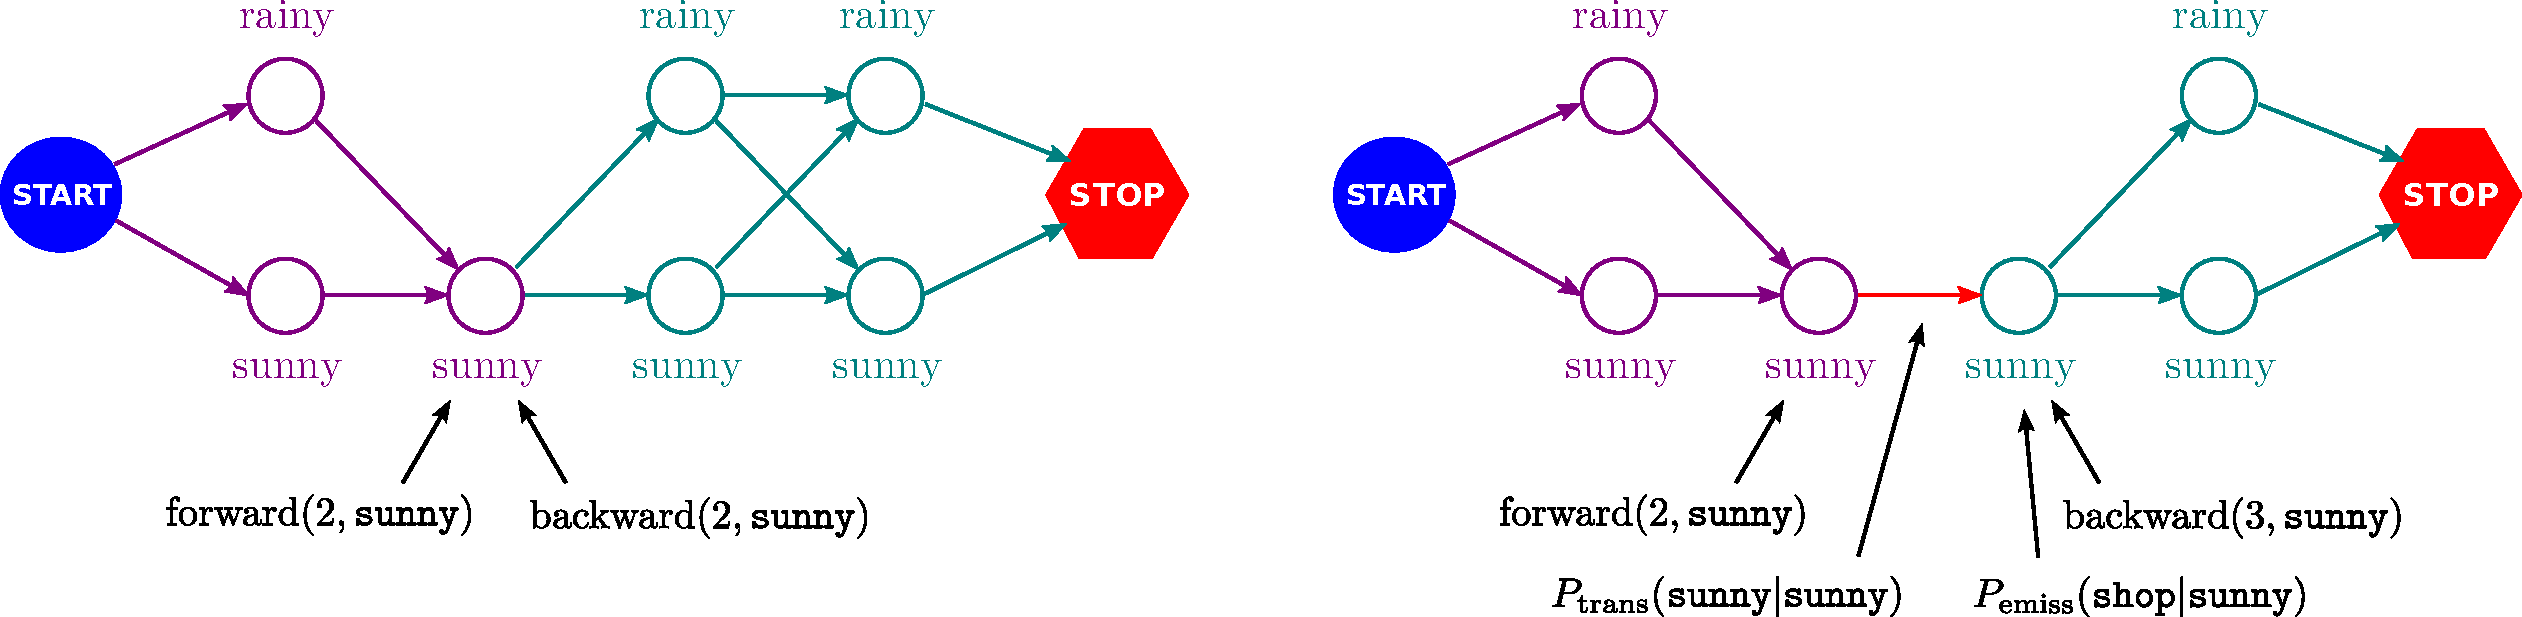
\includegraphics[width=1\textwidth]{figs/sequences/posteriors}
\caption[Posterior Illustration.]{\label{fig:posteriors} A graphical representation of the components in the state and transition posteriors. Recall that the observation sequence is ``\texttt{walk walk shop clean}''.}
\end{center}
\end{figure}

%\begin{figure}
%\begin{center}
%\begin{tabular}{cc}
%
%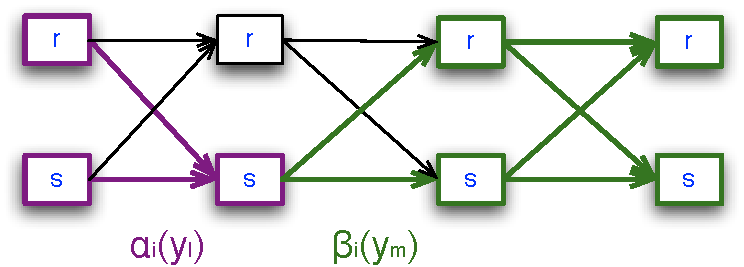
\includegraphics[scale=.5]{figs/sequences/statePost}
%& 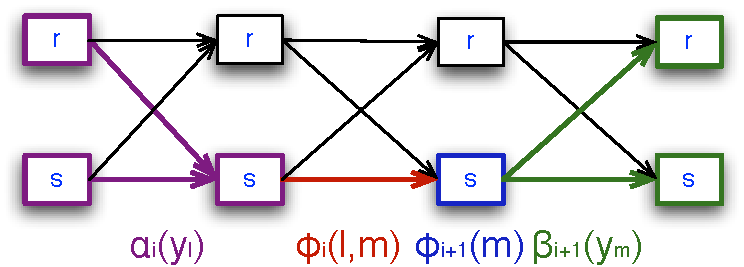
\includegraphics[scale=.5]{figs/sequences/transPost}\\
%\end{tabular}
%\caption[Posterior Illustration.]{\label{fig:posteriors} A graphical representation of the components in the state and transition posteriors.}
%
%\end{center}
%\end{figure}

Using the state posteriors, we are ready to perform posterior
decoding. 
The strategy is to compute the state posteriors 
for each position $i \in \{1,\ldots,N\}$
and each state $c_k \in \statevocab$, and 
then pick the arg-max at each position:
\begin{equation}
{\widehat y_i} := \argmax_{y_i \in \statevocab} P(Y_i=y_i| X=x).
\end{equation}

%Algorithm \ref{alg:pd} shows the posterior decoding algorithm.

%\begin{algorithm}[t]
%   \caption{Posterior Decoding algorithm \label{alg:pd}}
%\begin{algorithmic}[1]
%   \STATE {\bfseries input:} The forward and backward probabilities
%       $\alpha$ and $\beta$.
%   \STATE  \emph{Compute Likelihood}: Compute the likelihood of the
%   sentence
%   \STATE $L = 0$
%   \FOR{$\hv_l \in \hvocab$ }
%   \STATE $\marginal = \marginal + \alpha_N(\hv_l)$
%   \ENDFOR 
%   \STATE $\hat \hseq = []$
%    \FOR{$i=1$ {\bfseries to} $N$}
%    \STATE $max = 0$
%     \FOR{$\hv_l \in \hvocab$ }
%     \STATE $\gamma_i(\hv_l)  =  \frac{\alpha_i(\hv_l)
%       \beta_i(\hv_l)}{\marginal}$
%     \IF {$\gamma_i(\hv_l) > max$}
%     \STATE $max = \gamma_i(\hv_l)$
%     \STATE $\hat  y_i = \hv_l$
%     \ENDIF
%     \ENDFOR 
%     \ENDFOR 
%   \STATE \textbf{output:} the posterior path $\hat \hseq$
%\end{algorithmic}
%\end{algorithm}


\newpage
\begin{exercise}
%Given the node and edge posterior formulas \ref{eq::nodePosterior},\ref{eq::edgePosterior} and the
%  forward and backward formulas \ref{eq::forward},\ref{eq::backward}, convince yourself that formulas
%  \ref{eq::nodePosterior2},\ref{eq::edgePosterior2} are correct. 

Compute the node posteriors for the first training sequence (use the provided \emph{compute\_posteriors} function), and look at
the output. Note that the state posteriors are a proper
probability distribution (the lines of the result sum to 1).

\begin{python}
initial_scores, transition_scores, final_scores, emission_scores = hmm.compute_scores(simple.train.seq_list[0])
state_posteriors, _, _ = hmm.compute_posteriors(initial_scores,
                                                transition_scores,
                                                final_scores,
                                                emission_scores)
print state_posteriors

[[ 0.95738152  0.04261848]
 [ 0.75281282  0.24718718]
 [ 0.26184794  0.73815206]
 [ 0.          1.        ]]
\end{python}
\end{exercise}

\begin{exercise}
Run the posterior decode on the first test sequence, and evaluate it.
\begin{python}
y_pred = hmm.posterior_decode(simple.test.seq_list[0])
print "Prediction test 0:", y_pred

walk/rainy walk/rainy shop/sunny clean/sunny

print "Truth test 0:", simple.test.seq_list[0]

walk/rainy walk/sunny shop/sunny clean/sunny 
\end{python}

Do the same for the second test sequence:
\begin{python}
y_pred = hmm.posterior_decode(simple.test.seq_list[1])
print "Prediction test 1:", y_pred

clean/rainy walk/rainy tennis/rainy walk/rainy 

print "Truth test 1:", simple.test.seq_list[1]

clean/sunny walk/sunny tennis/sunny walk/sunny 
\end{python}

What is wrong? Note the observations for the second test sequence: the
observation {\tt tennis} was never seen at training time, so the probability for
it will be zero (no matter what state). This will make all possible state
sequences have zero probability.
As seen in the previous lecture, this is a problem with generative
models, which can be corrected using smoothing (among other
options).

Change the \emph{train\_supervised} method to add smoothing:
\begin{python}
def train_supervised(self,sequence_list, smoothing):
\end{python}

Try, for example, adding 0.1 to all the counts, and repeating this exercise with that smoothing. What do you observe?
\begin{python}
hmm.train_supervised(simple.train, smoothing=0.1)
y_pred = hmm.posterior_decode(simple.test.seq_list[0])
print "Prediction test 0 with smoothing:", y_pred

walk/rainy walk/rainy shop/sunny clean/sunny 

print "Truth test 0:", simple.test.seq_list[0]

walk/rainy walk/sunny shop/sunny clean/sunny

y_pred = hmm.posterior_decode(simple.test.seq_list[1])
print "Prediction test 1 with smoothing:", y_pred

clean/sunny walk/sunny tennis/sunny walk/sunny 

print "Truth test 1:", simple.test.seq_list[1]

clean/sunny walk/sunny tennis/sunny walk/sunny 
\end{python}
\end{exercise}

%Note that if you use smoothing when training, the sanity checks mentioned at the start of this chapter are no longer true. For example, the sum of all the transition counts is no longer equal to the number of tokens -- it is larger.

%\begin{exercise}
%Change the function you just created \emph{ def
%  sanity\_check\_counts(self,seq\_list):} to account for smoothing. Make
%sure it works properly.
%
%\begin{python}
%In []: run sequences/hmm.py
%In []: hmm = HMM(simple)
%In []: hmm.collect_counts_from_corpus(simple.train,smoothing=0.1)
%In []: hmm.sanity_check_counts(simple.train,smoothing=0.1)
%Init Counts match
%Final Counts match
%Transition Counts match
%Observations Counts match
%\end{python}
%\end{exercise}


\subsection{Viterbi Decoding}\label{viterbi}


\textbf{Viterbi decoding} consists in
picking the best global hidden state sequence 
$\widehat{y}$
as follows: 
\begin{equation}
\widehat{y} = \argmax_{y \in \statevocab^N} P(Y=y|X=x) = \argmax_{y \in \statevocab^N} P(X=x,Y=y).
\end{equation}

The Viterbi algorithm 
is very similar to the forward procedure of the FB algorithm,
making use of the same trellis structure to efficiently represent the exponential number of sequences without prohibitive computation costs. In fact, the only
difference from the forward-backward algorithm is in the recursion
\ref{forwardRecursion} where instead of \emph{summing} over all possible 
hidden states, we take their \emph{maximum}.

\begin{equation}
\label{eq::viterbi}
\mathbf{Viterbi }\;\;\;\;  \mathrm{viterbi}(i, y_i) = \max_{y_1...y_{i-1}} P(Y_1=y_1,\ldots Y_i = y_i , X_1=x_1,\ldots, X_i=x_i)
\end{equation}
The Viterbi trellis represents the path with maximum probability in
position
$i$ when we are in state $Y_i=y_i$ and that we have observed $x_1,\ldots,x_i$
up to that position. The Viterbi algorithm is defined by the
following recurrence: 
\begin{eqnarray}
\mathrm{viterbi}(1, c_k) &=& P_{\mathrm{init}}(c_k|\text{\tt start}) \times 
P_{\mathrm{emiss}}(x_1 | c_k)
 \\
 \mathrm{viterbi}(i, c_k) &=& \left( \displaystyle \max_{c_l \in \statevocab} P_{\mathrm{trans}}(c_k | c_l) \times \mathrm{viterbi}(i-1, c_l) \right) \times P_{\mathrm{emiss}}(x_i | c_k)  \label{viterbiRecursion}
 \\
 \mathrm{backtrack}(i, c_k) &=& \left( \displaystyle \argmax_{c_l \in \statevocab} P_{\mathrm{trans}}(c_k | c_l) \times \mathrm{viterbi}(i-1, c_l) \right) 
 \\
  \mathrm{viterbi}(N+1, \text{\tt stop}) &=& \max_{c_l \in \statevocab} P_{\mathrm{final}}(\text{\tt stop} | c_l) \times \mathrm{viterbi}(N, c_l)
 \\
  \mathrm{backtrack}(N+1, \text{\tt stop}) &=& \argmax_{c_l \in \statevocab} P_{\mathrm{final}}(\text{\tt stop} | c_l) \times \mathrm{viterbi}(N, c_l).
\end{eqnarray}


%\begin{eqnarray}
%\delta_1(\hv_l) &=& \phi_1(l) \\
%\delta_i(\hv_l) &=& \left[ \max_{y_1 ... y_i} \phi_{i-1,i}(m,l)
%  \delta_{i-1}(\hv_m) \right] \phi_i(l) \label{viterbiRecursion} \\
%\psi_{i}(\hv_l) &=& \left[ \argmax_{y_1 ... y_i} \phi_{i-1,i}(m,l)
%  \delta_{i-1}(\hv_m) \right]
%%\phi_{(i-1)}(m,l)  \delta_{i-1}(\hv_m) \right] \phi_i(l) \label{viterbiBackpointers}
%\end{eqnarray}

Algorithm \ref{alg:viterbi} shows the pseudo code for the Viterbi algorithm.
Note the similarity with the forward algorithm.
The only differences are:
\begin{itemize}
\item Maximizing instead of summing;
\item Keeping the argmax's to backtrack.
\end{itemize}

%\begin{algorithm}[t]
%   \caption{Viterbi algorithm \label{alg:viterbi}}
%\begin{algorithmic}[1]
%   \STATE {\bfseries input:} sentence $\sent$, parameters $\theta$
%        \STATE  \emph{Forward pass}: compute the maximum paths for
%        every end state
%        \STATE \emph{Initialization}
%        \FOR{$\hv_l \in \hvocab$ }
%        \STATE $\delta_1(\hv_l) = \phi_1(\hv_l)$
%        \ENDFOR 
%        \FOR{$i=2$ {\bfseries to} $N$}
%         \FOR{$\hv_l \in \hvocab$ }
%                 \STATE $\delta_i(\hv_l) = \left[ \displaystyle
%                   \max_{m  \in \hvocab} \phi_{i-1,i}(m,l)
%                   \delta_{i-1}(\hv_m) \right] \phi_i(l)$
%                 \STATE $\psi_{i}(\hv_l) = m$
%         \ENDFOR 
%        \ENDFOR 
%       %\STATE \emph{Terminate}:
%       \STATE 
%  $\max_{y \in \statevocab^N} P(X=x,Y=y) := \max_{c_l \in \statevocab} P_{\mathrm{final}}(\text{\tt stop} | c_l) \times \mathrm{viterbi}(N, c_l)$
%  	   \STATE 
%       \STATE \emph{Backward pass}: Build the most likely path
%	  \STATE $\widehat{y}_i = \argmax_{c_l \in \statevocab} P_{\mathrm{final}}(\text{\tt stop} | c_l) \times \mathrm{viterbi}(N, c_l)$ 
%	   \FOR{$i=N-1$ {\bfseries to} 1}
%        \STATE $\widehat{y_i} = \mathrm{backtrack}(i+1, \widehat{y}_{i+1})$
%        \ENDFOR 
%       \STATE \textbf{output:} the viterbi path $\widehat{y}$
%\end{algorithmic}
%\end{algorithm}

\begin{algorithm}[t]
   \caption{Viterbi algorithm \label{alg:viterbi}}
\begin{algorithmic}[1]
   \STATE {\bfseries input:} sequence $x_1,\ldots,x_N$, scores $P_{\mathrm{init}}, P_{\mathrm{trans}}, P_{\mathrm{final}}, P_{\mathrm{emiss}}$
        \STATE  \emph{Forward pass}: Compute the best paths for every end state
        \STATE \emph{Initialization}
        \FOR{$c_k \in \statevocab$ }
        \STATE $\mathrm{viterbi}(1,c_k) = P_{\mathrm{init}}(c_k|\text{\tt start}) \times 
P_{\mathrm{emiss}}(x_1 | c_k)$
        \ENDFOR 
        \FOR{$i=2$ {\bfseries to} $N$}
         \FOR{$c_k \in \statevocab$ }
          \STATE $\mathrm{viterbi}(i, c_k) = \left( \displaystyle \max_{c_l \in \statevocab} P_{\mathrm{trans}}(c_k | c_l) \times \mathrm{viterbi}(i-1, c_l) \right) \times P_{\mathrm{emiss}}(x_i | c_k)$
          \STATE $\mathrm{backtrack}(i, c_k) = \left( \displaystyle \argmax_{c_l \in \statevocab} P_{\mathrm{trans}}(c_k | c_l) \times \mathrm{viterbi}(i-1, c_l) \right)$
         \ENDFOR 
        \ENDFOR 
       \STATE 
  $\max_{y \in \statevocab^N} P(X=x,Y=y) := \max_{c_l \in \statevocab} P_{\mathrm{final}}(\text{\tt stop} | c_l) \times \mathrm{viterbi}(N, c_l)$        
        \STATE
       \STATE \emph{Backward pass}: backtrack to obtain the most likely path 
	  \STATE $\widehat{y}_N = \argmax_{c_l \in \statevocab} P_{\mathrm{final}}(\text{\tt stop} | c_l) \times \mathrm{viterbi}(N, c_l)$ 
	   \FOR{$i=N-1$ {\bfseries to} 1}
        \STATE $\widehat{y_i} = \mathrm{backtrack}(i+1, \widehat{y}_{i+1})$
        \ENDFOR 
       \STATE \textbf{output:} the viterbi path $\widehat{y}$.
\end{algorithmic}
\end{algorithm}

\section{Assignment}

With the previous theoretical background, you have the necessary tools to solve today's assignment.

\begin{exercise}
Implement a method 
for performing Viterbi decoding in 
file {\tt sequence\_classification\_decoder.py}.
\begin{python}
        def run_viterbi(self, initial_scores, transition_scores, final_scores, emission_scores):
\end{python}
Hint: look at the implementation of {\tt run\_forward}. Also check the help for the numpy methods max and argmax.

This method will be called 
by 
\begin{python}
def viterbi_decode(self, sequence)
\end{python}
in the module {\tt sequence\_classifier.py}.
%
%posterior decoding (the function \emph{posterior\_decode}) for reference.

Test your method on both test sequences and compare the results with
the ones given.
\begin{python}
hmm.train_supervised(simple.train, smoothing=0.1)
y_pred, score = hmm.viterbi_decode(simple.test.seq_list[0])
print "Viterbi decoding Prediction test 0 with smoothing:", y_pred, score

walk/rainy walk/rainy shop/sunny clean/sunny  -6.02050124698

print "Truth test 0:", simple.test.seq_list[0]

walk/rainy walk/sunny shop/sunny clean/sunny 

y_pred, score = hmm.viterbi_decode(simple.test.seq_list[1])
print "Viterbi decoding Prediction test 1 with smoothing:", y_pred, score

clean/sunny walk/sunny tennis/sunny walk/sunny  -11.713974074

print "Truth test 1:", simple.test.seq_list[1]

clean/sunny walk/sunny tennis/sunny walk/sunny 
\end{python}

Note: since we didn't run the \emph{train\_supervised} method again, we are still using the result of the training using smoothing. Therefore, you should compare these results to the ones of posterior decoding with smoothing.

\end{exercise}




%%% Local Variables: 
%%% mode: latex
%%% TeX-master: "../../guide"
%%% End: 


\section{\label{pos-tagging} Part-of-Speech Tagging (POS)}
Part-of-Speech (PoS) tagging is one of the most important NLP tasks. The
task is to assign each word a grammatical category, or Part-of-Speech, \emph{i.e.} noun,
verb, adjective,... Recalling the defined notation, $\vocab$ is a 
vocabulary of word types, and 
$\statevocab$ is the set of Part-of-Speech tags.

In English, using the Penn Treebank (PTB) corpus \citep{pennTreeBank}, the current
state of the art for part of speech tagging is around 97\% for a
variety of methods.

In the rest of this class we will use a subset of the PTB corpus, but
instead of using the original 45 tags we will use a reduced tag set of
12 tags, to make the algorithms faster for the
class. In this task, $x$ is a sentence (\emph{i.e.}, a sequence of word tokens) and $y$
is the sequence of possible PoS tags.

The first step is to load the corpus. We will start by loading
1000 sentences for training and 1000 sentences both for development and
testing. Then we train the HMM model by maximum likelihood estimation.
\begin{python}
import lxmls.readers.pos_corpus as pcc
corpus = pcc.PostagCorpus()
train_seq = corpus.read_sequence_list_conll("data/train-02-21.conll",max_sent_len=15,max_nr_sent=1000)
test_seq = corpus.read_sequence_list_conll("data/test-23.conll",max_sent_len=15,max_nr_sent=1000)
dev_seq = corpus.read_sequence_list_conll("data/dev-22.conll",max_sent_len=15,max_nr_sent=1000)
hmm = hmmc.HMM(corpus.word_dict, corpus.tag_dict)
hmm.train_supervised(train_seq)
hmm.print_transition_matrix()
\end{python}


Look at the transition probabilities of the trained model
%\begin{python}
%In []: import matplotlib.pyplot as plt
%In []: hmm.transition_probs
%\end{python}
 (see
Figure \ref{fig:transProbs}), and see if they match your intuition
about the English language (e.g. adjectives tend to come before nouns).

\begin{figure}[h!]
\centering
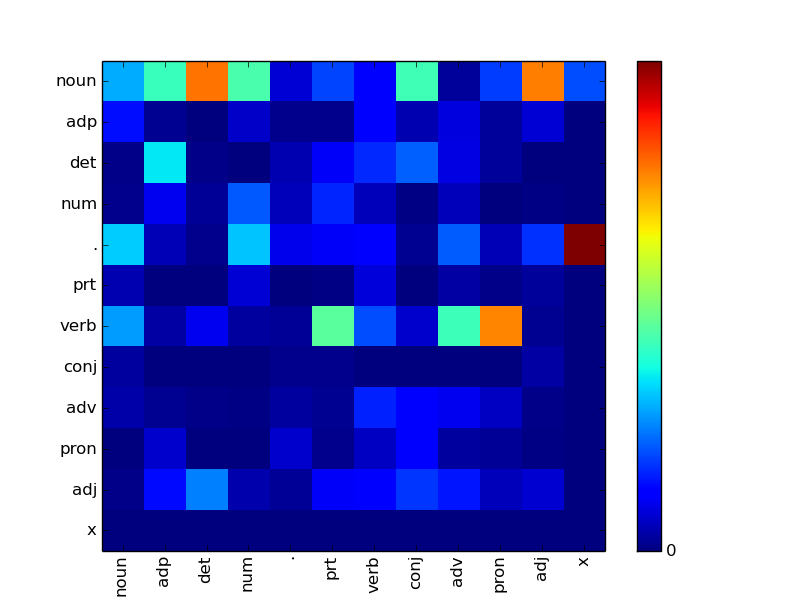
\includegraphics[scale=.5]{figs/sequences/transition_probs}
\caption{\label{fig:transProbs} Transition probabilities of the
trained model. Each column is the previous state and row is the current
state. Note the high probability of having Noun after Determinant or Adjective, or of having Verb after Nouns or Pronouns, as expected.}
\end{figure}

\begin{exercise}
Test the model using both posterior decoding and Viterbi decoding on
both the train and test set, using the methods in class HMM:
\begin{python}
viterbi_pred_train = hmm.viterbi_decode_corpus(train_seq)
posterior_pred_train = hmm.posterior_decode_corpus(train_seq)
eval_viterbi_train =   hmm.evaluate_corpus(train_seq, viterbi_pred_train)
eval_posterior_train =  hmm.evaluate_corpus(train_seq, posterior_pred_train)
print "Train Set Accuracy: Posterior Decode \%.3f, Viterbi Decode: \%.3f"\%(eval_posterior_train,eval_viterbi_train)

Train Set Accuracy: Posterior Decode 0.985, Viterbi Decode: 0.985

viterbi_pred_test = hmm.viterbi_decode_corpus(test_seq)
posterior_pred_test = hmm.posterior_decode_corpus(test_seq)
eval_viterbi_test =   hmm.evaluate_corpus(test_seq,viterbi_pred_test)
eval_posterior_test = hmm.evaluate_corpus(test_seq,posterior_pred_test)
print "Test Set Accuracy: Posterior Decode \%.3f, Viterbi Decode: \%.3f"\%(eval_posterior_test,eval_viterbi_test)

Test Set Accuracy: Posterior Decode 0.350, Viterbi Decode: 0.509
\end{python}
What do you observe? Remake the previous exercise but now train the HMM
using smoothing. Try different values (0,0.1,0.01,1) and report the results on the
train and development set. (Use function
\emph{pick\_best\_smoothing}).


\begin{python}
best_smoothing = hmm.pick_best_smoothing(train_seq, dev_seq, [10,1,0.1,0])

Smoothing 10.000000 --  Train Set Accuracy: Posterior Decode 0.731, Viterbi Decode: 0.691
Smoothing 10.000000 -- Test Set Accuracy: Posterior Decode 0.712, Viterbi Decode: 0.675
Smoothing 1.000000 --  Train Set Accuracy: Posterior Decode 0.887, Viterbi Decode: 0.865
Smoothing 1.000000 -- Test Set Accuracy: Posterior Decode 0.818, Viterbi Decode: 0.792
Smoothing 0.100000 --  Train Set Accuracy: Posterior Decode 0.968, Viterbi Decode: 0.965
Smoothing 0.100000 -- Test Set Accuracy: Posterior Decode 0.851, Viterbi Decode: 0.842
Smoothing 0.000000 --  Train Set Accuracy: Posterior Decode 0.985, Viterbi Decode: 0.985
Smoothing 0.000000 -- Test Set Accuracy: Posterior Decode 0.370, Viterbi Decode: 0.526

hmm.train_supervised(train_seq, smoothing=best_smoothing)
viterbi_pred_test = hmm.viterbi_decode_corpus(test_seq)
posterior_pred_test = hmm.posterior_decode_corpus(test_seq)
eval_viterbi_test =   hmm.evaluate_corpus(test_seq, viterbi_pred_test)
eval_posterior_test = hmm.evaluate_corpus(test_seq, posterior_pred_test)
print "Best Smoothing \%f --  Test Set Accuracy: Posterior Decode \%.3f, Viterbi Decode: \%.3f"%(best_smoothing,eval_posterior_test,eval_viterbi_test)

Best Smoothing 0.100000 --  Test Set Accuracy: Posterior Decode 0.837, Viterbi Decode: 0.827
\end{python}


Perform some error analysis to understand were the errors are coming
from. You can start by visualizing the confusion matrix (true tags vs
predicted tags). You should get something like what is shown in Figure~\ref{fig:cmuns}.

\begin{python}
import lxmls.sequences.confusion_matrix as cm
import matplotlib.pyplot as plt
confusion_matrix = cm.build_confusion_matrix(test_seq.seq_list, viterbi_pred_test, len(corpus.tag_dict), hmm.get_num_states())
cm.plot_confusion_bar_graph(confusion_matrix, corpus.tag_dict, xrange(hmm.get_num_states()), 'Confusion matrix')
plt.show()
\end{python}

\begin{figure}[h!]
\centering
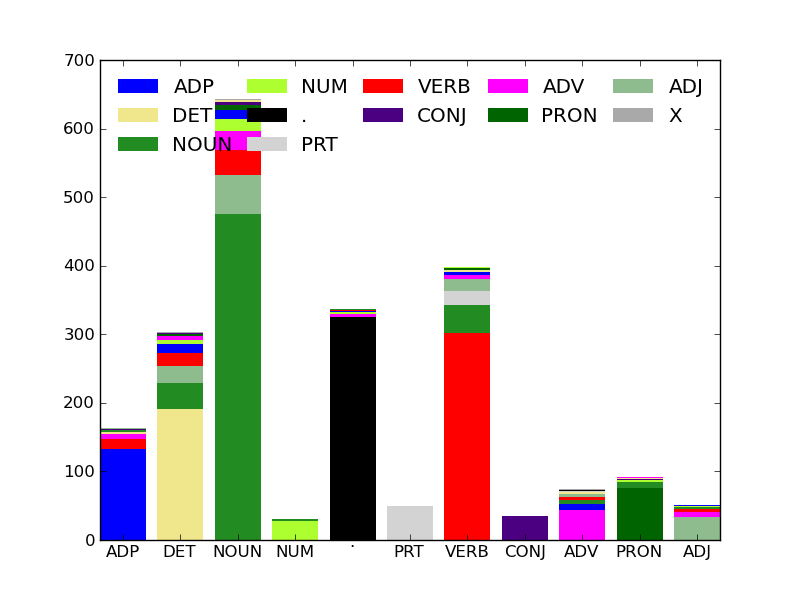
\includegraphics[scale=.4]{figs/sequences/cm_sup.png}
\caption{\label{fig:cmuns} Confusion Matrix for the previous
  example. Predicted tags are columns and the true tags corresponds to
  the constituents of each column.}
\end{figure}

\end{exercise}


%\begin{exercise}
%Implement a function that produces the accuracy for rare words vs
%common words. Use you own definition of rare word.
%
%Can you come up with other error analysis methods? Which?
%
%\end{exercise}

%\begin{exercise}
%So far we have only worked with a limited dataset of 1000 words. Try increasing the number of sentences to 10000. What do you observe?
%\end{exercise}


%\section{Unsupervised Learning of HMMs}
%
%\afm{explain here the EM algorithm}
%
%\begin{python}
%
%Initial accuracy: 0.303638
%Iter: 1 Log Likelihood: -101824.763927
%Iter: 1 Accuracy: 0.305441
%Iter: 2 Log Likelihood: -78057.108346
%Iter: 2 Accuracy: 0.321976
%Iter: 3 Log Likelihood: -77813.725501
%Iter: 3 Accuracy: 0.357451
%Iter: 4 Log Likelihood: -77192.947674
%Iter: 4 Accuracy: 0.385109
%Iter: 5 Log Likelihood: -76191.800849
%Iter: 5 Accuracy: 0.392123
%Iter: 6 Log Likelihood: -75242.572729
%Iter: 6 Accuracy: 0.391121
%Iter: 7 Log Likelihood: -74392.892496
%Iter: 7 Accuracy: 0.404249
%Iter: 8 Log Likelihood: -73357.542833
%Iter: 8 Accuracy: 0.399940
%Iter: 9 Log Likelihood: -72135.182778
%Iter: 9 Accuracy: 0.399238
%Iter: 10 Log Likelihood: -70924.246230
%Iter: 10 Accuracy: 0.395430
%Iter: 11 Log Likelihood: -69906.561800
%Iter: 11 Accuracy: 0.394328
%Iter: 12 Log Likelihood: -69140.228623
%Iter: 12 Accuracy: 0.390821
%Iter: 13 Log Likelihood: -68541.416423
%Iter: 13 Accuracy: 0.391522
%Iter: 14 Log Likelihood: -68053.456865
%Iter: 14 Accuracy: 0.389117
%Iter: 15 Log Likelihood: -67667.318961
%Iter: 15 Accuracy: 0.386411
%Iter: 16 Log Likelihood: -67337.685686
%Iter: 16 Accuracy: 0.385409
%Iter: 17 Log Likelihood: -67054.571821
%Iter: 17 Accuracy: 0.385409
%Iter: 18 Log Likelihood: -66769.973881
%Iter: 18 Accuracy: 0.385409
%Iter: 19 Log Likelihood: -66442.608458
%Iter: 19 Accuracy: 0.385409
%
%\end{python}



%\section{\label{hmm_special_state} HMM Initial and Final State}
%\input{pages/sequences/init_final_hmm.tex}

%\section{\label{hmm} Second order HMM}
%
\subsection{State Expansion}

The ideia here is to expand the states and use the same inference
procedures as those of the HMM.



\subsection{Modelling second order}

Here we use the original states and we derive new inference procedures....

\begin{eqnarray*}
\alpha_{t=2}(1) &=& P(y_{t=2} = 1,x_0,x_1,x_2) = \sum_{b \in \hvocab}
\sum_{a\in \hvocab} P(y_{t=2} = 1,x_0,x_1,x_2, y_{t=0}=a,y_{t=1}=b)\\
\alpha_{t=2}(1) &=& \sum_{b \in \hvocab}
\sum_{a\in \hvocab}
p(x_2 |  y_{t=2}) p(y_{t=2} | y_{t=1} =b ,y_{t=0}=a)  p(x_1 |  y_{t=1}
=b) p(y_{t=1} =b| y_{t=0}=a)\\
&*&  p(x_0 |  y_{t=0}=a) p(y_{t=0}=a) \\
\alpha_{t=2}(1) &=& \sum_{b \in \hvocab}
\sum_{a\in \hvocab}
p(x_2 |  y_{t=2}) p(y_{t=2} | y_{t=1} = b,y_{t=0} = a)  p(x_1 |
y_{t=1} = b) p(y_{t=1} = b| y_{t=0} = a)  \mathbf{p(x_0 ,  y_{t=0} = a) }\\
\alpha_{t=2}(1) &=& \sum_{b \in \hvocab}
\sum_{a\in \hvocab}
p(x_2 |  y_{t=2}) p(y_{t=2} | y_{t=1} = b,y_{t=0} = a)  p(x_1 |
y_{t=1} = b) p(y_{t=1} = b| y_{t=0} = a)  \alpha_{t=0}(a) \\
\alpha_{t=2}(1) &=& \sum_{b \in \hvocab}
\sum_{a\in \hvocab}
p(x_2 |  y_{t=2}) p(y_{t=2} | y_{t=1} = b,y_{t=0} = a)  p(x_1 ,
y_{t=1} = b | y_{t=0} = a)  \alpha_{t=0}(a) \\
\alpha_{t=2}(1) &=& \sum_{b \in \hvocab}
\sum_{a\in \hvocab}
p(x_2 |  y_{t=2}) p(y_{t=2} | y_{t=1} = b,y_{t=0} = a)  \mathbf{p(x_1 ,
y_{t=1} = b ,x_0 ,  y_{t=0} = a) }
\end{eqnarray*}

%%% Local Variables: 
%%% mode: latex
%%% TeX-master: "../../guide"
%%% End: 


%%% Local Variables: 
%%% mode: latex
%%% TeX-master: "../../guide.tex"
%%% End: 
